% Prova del 01/02/1970, esercizio 1: riflessione di un urto obliquo su una lastra piana con corrente a M = 1,3.
% Numeri e figure: calcoli.py (stessa cartella).

\documentclass[11pt,a4paper]{article}

\usepackage[T1]{fontenc}
\usepackage[utf8]{inputenc}
\usepackage[italian]{babel}
\usepackage{amsmath,amssymb}
\usepackage[a4paper,margin=2.4cm]{geometry}
\usepackage{array}
\usepackage{siunitx}
\usepackage{booktabs}
\usepackage{graphicx}
\usepackage{float}
\usepackage{hyperref}

\hypersetup{hidelinks}
\setlength{\parindent}{0pt}
\setlength{\parskip}{4pt}
\allowdisplaybreaks
\graphicspath{{figure/}}
\sisetup{output-decimal-marker={,}, group-separator={\,}, per-mode=symbol,
         exponent-product=\cdot, range-phrase={\text{--}}}

\newcommand{\Cp}{C^{+}}
\newcommand{\Cm}{C^{-}}

\title{Gasdinamica -- Prova del 01/02/1970, esercizio 1\\[2pt]
\large Riflessione di un urto obliquo su una lastra piana a $M=1{,}3$}
\author{}
\date{}

\begin{document}
\maketitle

\section*{Traccia}
Una corrente uniforme supersonica, stazionaria e bidimensionale a $M=1{,}3$ scorre lungo una lastra piana su cui
incide un urto obliquo. Definire la relativa polare pressione--deviazione e determinare le diverse riflessioni
possibili dell'urto obliquo (modello di gas ideale). Descrivere le diverse riflessioni individuate nel piano fisico
$(x,y)$ (valutazione 13/30).

\begin{figure}[H]
  \centering
  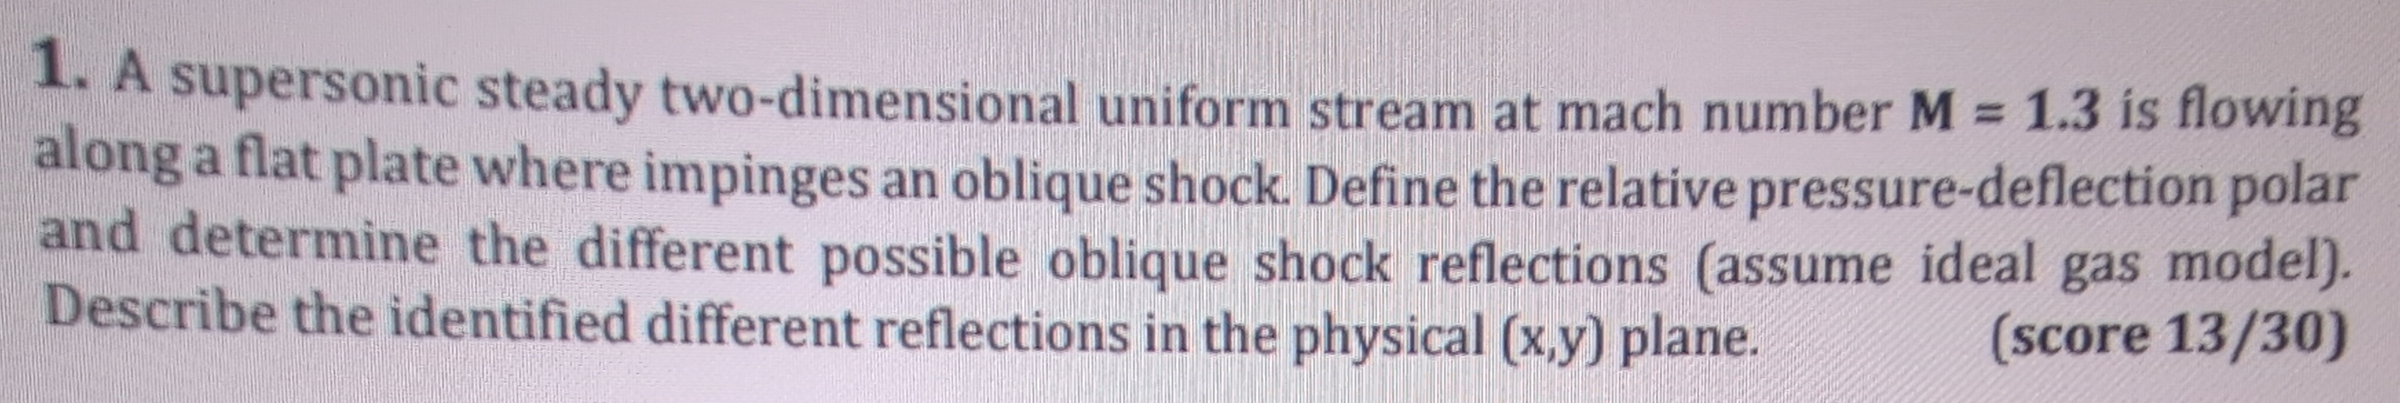
\includegraphics[width=0.85\textwidth]{originale.png}
  \caption{Traccia originale.}
\end{figure}

%==============================================================================
\section{Lettura del testo e dati}
La corrente 1 è parallela alla lastra ($\theta_1=0$). Un urto obliquo, generato altrove (per esempio da un cuneo
posto sopra la lastra), la investe e la devia verso la lastra di un angolo $\theta_I$; la lastra impone di nuovo
$\theta=0$, e il modo in cui ciò avviene è la ``riflessione''. La traccia \textbf{non assegna} l'intensità
dell'urto incidente: la interpreto come richiesta di classificare le riflessioni possibili al variare della
deviazione $\theta_I$ (equivalentemente dell'angolo d'urto $\sigma_I$), per $M_1=1{,}3$ fissato. Il dato
caratterizzante è il Mach \textbf{basso}: la polare di $M_1=1{,}3$ è piccola e quella riflessa ancora di più.

\begin{table}[H]
  \centering
  \begin{tabular}{lll}
    \toprule
    Grandezza & Valore & Note \\
    \midrule
    $\gamma$ & \num{1.4} & gas ideale, aria (non indicato) \\
    $M_1$, $\theta_1$, $p_1$ & $1{,}3$, \ang{0}, 1 & corrente indisturbata, pressioni riferite a $p_1$ \\
    $\theta_I$ & parametro & deviazione imposta dall'urto incidente, $0<\theta_I<\theta_{\max}(M_1)$ \\
    \bottomrule
  \end{tabular}
  \caption{Dati del problema.}
\end{table}

La stessa traccia è nel catalogo come B69-E01 (25/01/2023).

%==============================================================================
\section{Modello e ipotesi}
\begin{enumerate}
\item \textbf{Flusso piano, stazionario, non viscoso, gas perfetto con $\gamma=1{,}4$.} Trascuro lo strato limite
  sulla lastra e la sua interazione con l'urto.
\item \textbf{Urti rettilinei e stati uniformi} fra di essi: ogni urto è descritto dalle relazioni di
  Rankine--Hugoniot dell'urto obliquo, cioè da un punto della polare $p$--$\theta$ dello stato a monte.
\item \textbf{Regioni supersoniche} dove si applica il modello stazionario 2D iperbolico: la riflessione è
  determinata localmente nel punto d'impatto solo finché le regioni 2 e 3 sono supersoniche (da verificare, §8).
  Una regione subsonica riceve informazione da valle e la struttura non è più determinata dalle sole polari.
\item \textbf{Urto incidente sul ramo debole}: il campo è esterno e nessuna contropressione impone il ramo forte;
  stessa scelta per il riflesso, salvo discutere la seconda intersezione.
\end{enumerate}

%==============================================================================
\section{Analisi qualitativa}
\textbf{Urto incidente.} Viene dall'alto: è un'onda $\Cm$ di compressione che devia la corrente di $-\theta_I$,
verso la lastra, e porta lo stato 2 sul ramo debole della polare di 1.

\textbf{Onda riflessa.} Dietro l'incidente la corrente punta contro la lastra, che impone $\theta=0$: dalla lastra
nasce un'onda $\Cp$ che deve ruotare la corrente di $+\theta_I$. Su una parete un'onda si riflette con la
\textbf{stessa natura}: il riflesso è una compressione, cioè un urto, e la pressione sulla lastra cresce due
volte ($p_3>p_2>p_1$).

\textbf{Perché il Mach basso è decisivo.} Il riflesso deve produrre la stessa deviazione $\theta_I$ partendo da
$M_2<M_1$, quindi con una polare più piccola: esiste solo se $\theta_I\le\theta_{\max}(M_2)$. Crescendo $\theta_I$,
$M_2$ cala e $\theta_{\max}(M_2)$ cala anch'esso: c'è un angolo di distacco $\theta_D$ oltre il quale la riflessione
regolare (RR) è impossibile. A $M_1=1{,}3$ la polare di 1 arriva solo a $\theta_{\max}=\ang{6.66}$, quindi tutta la
fenomenologia sta in pochi gradi. Oltre $\theta_D$ si deve verificare se esiste una riflessione di Mach (MR) a tre
urti: incidente, riflesso e gambetto quasi normale, con una linea di scorrimento uscente dal punto triplo.

%==============================================================================
\section{Topologia del campo}
Gli stati sono numerati come d'uso: 1 a monte, 2 dopo l'incidente, 3 dopo il riflesso, 4 dietro il gambetto
(o dietro il tratto normale dell'urto).
\begin{itemize}
\item \textbf{RR}: due urti rettilinei che si incontrano sulla lastra in un punto; regioni uniformi 1, 2, 3, con
  $\theta_1=\theta_3=0$ e $\theta_2=-\theta_I$.
\item \textbf{MR}: punto triplo staccato dalla lastra; fra il punto triplo e la lastra un gambetto quasi normale,
  dietro il quale la regione 4 è subsonica; la linea di scorrimento separa 3 da 4 con $p_3=p_4$, $\theta_3=\theta_4$.
\item \textbf{Nessuna riflessione}: un solo urto, rettilineo lontano dalla lastra, che si incurva e la raggiunge
  perpendicolarmente; dietro il tratto quasi normale una sacca subsonica 4, chiusa da una linea sonica.
\end{itemize}
Quale di queste si realizza lo stabilisce il calcolo; le figure nel piano fisico sono in §10.

%==============================================================================
\section{Bilancio equazioni/incognite}
\textbf{RR.} Noto 2, l'urto riflesso ha un'incognita (il suo angolo $\sigma_R$) e una condizione, $\theta_3=0$: il
problema è chiuso ed equivale a intersecare la polare $\Cp$ di 2 con l'asse $\theta=0$. Una sola onda nasce dalla
parete e una sola condizione vi è imposta: il numero di condizioni al contorno coincide con le caratteristiche
entranti.

\textbf{MR (teoria dei tre urti).} Noto 2, incognite gli angoli del riflesso e del gambetto (cioè $p_3,\theta_3$ e
$p_4,\theta_4$, ciascuna coppia vincolata alla propria polare); condizioni sulla linea di scorrimento $p_3=p_4$,
$\theta_3=\theta_4$. Due equazioni in due incognite: graficamente, l'intersezione della polare $\Cp$ di 2 con il ramo
forte della polare di 1. Il bilancio è chiuso, ma la soluzione può non esistere.

%==============================================================================
\section{Scorciatoie fisiche}
\begin{itemize}
\item L'esistenza della RR non richiede di intersecare le polari: basta confrontare $\theta_I$ con
  $\theta_{\max}(M_2)$. Il limite $\theta_D$ è quindi la radice di $\theta_{\max}(M_2(\theta_I))=\theta_I$.
\item Il criterio di von Neumann (polari che si incontrano sull'asse $\theta=0$ nel punto d'urto normale di 1)
  richiede $p_3=p_{n1}$. Poiché $p_3$ cresce con $\theta_I$, basta confrontare il suo valore massimo, a $\theta_D$, con
  $p_{n1}$: se è minore, $\theta_N$ non esiste.
\item Per $\theta_I\to0$ le onde sono acustiche: ognuna dà $\Delta p/p\simeq\gamma M^2\theta/\sqrt{M^2-1}$ e la
  riflessione su parete \textbf{raddoppia} il salto, $p_3-p_1\simeq2(p_2-p_1)$: utile come controllo del calcolo.
\end{itemize}

%==============================================================================
\section{Calcolo}

\subsection*{a) Polare pressione--deviazione dello stato 1}
Attraverso un urto obliquo di angolo $\sigma$ si conserva la componente tangenziale della velocità e la normale
subisce il salto dell'urto normale con $M_{n1}=M_1\sin\sigma$. Da $V_t$ costante e dalla continuità,
$\tan(\sigma-\theta)/\tan\sigma=\rho_1/\rho_2=[(\gamma-1)M_{n1}^2+2]/[(\gamma+1)M_{n1}^2]$, da cui
\[
\tan\theta=2\cot\sigma\,\frac{M_1^2\sin^2\sigma-1}{M_1^2(\gamma+\cos2\sigma)+2},\qquad
\frac{p_2}{p_1}=1+\frac{2\gamma}{\gamma+1}\left(M_1^2\sin^2\sigma-1\right),\qquad
M_2=\frac{M_{n2}}{\sin(\sigma-\theta)} ,
\]
con $M_{n2}^2=(1+\delta M_{n1}^2)/(\gamma M_{n1}^2-\delta)$. Al variare di $\sigma$ da $\mu_1$ a \ang{90}, la coppia
$(\theta,p)$ descrive la polare (con $\pm\theta$ per le due famiglie). Punti notevoli per $M_1=1{,}3$:
\begin{itemize}
\item onda nulla: $\sigma=\mu_1=\arcsin(1/M_1)=\ang{50.3}$, $p/p_1=1$;
\item massima deviazione ($d\theta/d\sigma=0$): $\theta_{\max}=\ang{6.66}$ a $\sigma=\ang{69.4}$, $p/p_1=1{,}56$;
\item punto sonico ($M_2=1$): $\theta_s=\ang{6.32}$ a $\sigma=\ang{65.1}$, $p/p_1=1{,}46$;
\item urto normale: $\theta=0$, $p_{n1}/p_1=1{,}805$, $M=0{,}786$.
\end{itemize}
Il ramo debole va da $\mu_1$ al punto sonico; fra punto sonico e $\theta_{\max}$ è ancora ``debole'' ma con valle
subsonica.

\subsection*{b) Riflessione regolare: esempio a $\theta_I=\ang{2}$}
\textbf{Stato 2.} Dalla relazione $\theta$--$\sigma$--$M$ con $M_1$ e $\theta_I$, ramo debole:
\[
\sigma_I=\ang{53.5},\quad M_{n1}=1{,}045,\quad p_2/p_1=1{,}107,\quad M_2=1{,}22,\quad \theta_2=-\ang{2}.
\]
La polare di 2 arriva a $\theta_{\max}(M_2)=\ang{4.59}>\theta_I$: la RR esiste.

\textbf{Stato 3.} Stessa relazione con $M_2$ e deviazione $+\theta_I$ (onda $\Cp$, da $\theta_2=-\theta_I$ a
$\theta_3=0$), ramo debole. L'angolo $\sigma_R$ è misurato dalla direzione della corrente 2, quindi l'urto
riflesso forma con la lastra l'angolo $\varphi_R=\sigma_R-\theta_I$:
\[
\sigma_R=\ang{58.9},\quad \varphi_R=\ang{56.9},\quad M_{n2}=1{,}048,\quad p_3/p_2=1{,}115,\quad p_3/p_1=1{,}23,
\quad M_3=1{,}14 .
\]
La seconda intersezione della polare di 2 con $\theta=0$, sul ramo forte, dà $p_{3'}/p_1=1{,}73$, $M_{3'}=0{,}84$,
$\varphi_{R'}=\ang{82.6}$: richiederebbe una contropressione imposta a valle, assente in un campo esterno, e la
scarto.

\subsection*{c) Criterio di distacco e criterio sonico}
Ripetendo il calcolo al variare di $\theta_I$ (tabella~\ref{tab:rr}), $M_2$ diminuisce e la polare riflessa si
restringe. Il distacco è la radice di $\theta_{\max}(M_2(\theta_I))=\theta_I$, cioè la polare di 2 tangente all'asse
$\theta=0$:
\[
\theta_D=\ang{3.25}\quad(\sigma_I=\ang{55.8},\ M_2=1{,}17,\ p_2/p_1=1{,}18;\ \text{al distacco }p_3/p_1=1{,}54,\
M_3=0{,}96).
\]
Già un po' prima la regione 3 diventa subsonica: $M_3=1$ per $\theta_S=\ang{3.15}$ ($p_3/p_1=1{,}46$).

\begin{table}[H]
  \centering
  \begin{tabular}{cccccccc}
    \toprule
    $\theta_I$ & $\sigma_I$ & $p_2/p_1$ & $M_2$ & $\theta_{\max}(M_2)$ & $\varphi_R$ & $p_3/p_1$ & $M_3$ \\
    \midrule
    \ang{1}    & \ang{51.8} & 1,051 & 1,263 & \ang{5.64} & \ang{53.0} & 1,107 & 1,224 \\
    \ang{2}    & \ang{53.5} & 1,107 & 1,224 & \ang{4.59} & \ang{56.9} & 1,233 & 1,140 \\
    \ang{3}    & \ang{55.3} & 1,167 & 1,184 & \ang{3.52} & \ang{63.7} & 1,415 & 1,028 \\
    $\theta_S=\ang{3.15}$ & \ang{55.6} & 1,176 & 1,178 & \ang{3.36} & \ang{65.8} & 1,462 & 1,000 \\
    $\theta_D=\ang{3.25}$ & \ang{55.8} & 1,183 & 1,173 & \ang{3.25} & \ang{69.7} & 1,537 & 0,955 \\
    \bottomrule
  \end{tabular}
  \caption{Riflessione regolare (riflesso debole) al variare della deviazione dell'urto incidente.}
  \label{tab:rr}
\end{table}

\subsection*{d) Criterio di von Neumann}
Il massimo di $p_3$ sulla RR si ha al distacco: $p_3/p_1=1{,}54<p_{n1}/p_1=1{,}805$. La pressione dell'urto normale
di 1 non è mai raggiunta: le due polari non si incontrano mai sull'asse $\theta=0$ e \textbf{l'angolo di von Neumann
non esiste} a $M_1=1{,}3$. Manca quindi anche il dominio di doppia soluzione (isteresi RR/MR): sotto $\theta_D$ c'è
solo la RR.

\subsection*{e) Oltre il distacco: teoria dei tre urti}
Per $\theta_D<\theta_I<\theta_s(M_1)$ cerco l'intersezione della polare $\Cp$ di 2 con il ramo forte della polare di 1.
Esempio $\theta_I=\ang{5}$: $\sigma_I=\ang{60.0}$, $M_2=1{,}09$, $p_2/p_1=1{,}31$, $\theta_{\max}(M_2)=\ang{1.31}$. La
polare di 2 occupa solo $-\ang{6.31}\le\theta\le-\ang{3.69}$ e arriva al massimo a $p/p_1=1{,}60$ (urto riflesso
normale), mentre il ramo forte della polare di 1 a $\theta=-\ang{5}$ è a $p/p_1=1{,}73$. La polare riflessa è
\textbf{tutta interna} alla polare dell'urto incidente e non la interseca, se non nel punto 2; lo stesso accade per
ogni $\theta_I$ dell'intervallo. La teoria dei tre urti non ha soluzione: \textbf{a $M_1=1{,}3$ non esiste MR}.

Per $\theta_s(M_1)=\ang{6.32}<\theta_I<\theta_{\max}(M_1)=\ang{6.66}$ la regione 2 è già subsonica e non può esistere
un urto riflesso; per $\theta_I>\theta_{\max}(M_1)$ l'urto incidente stesso non può essere attaccato al corpo che lo
genera.

\subsection*{f) Configurazione oltre il distacco}
La polare riflessa non interseca né l'asse delle pressioni ($\theta=0$) né la polare dell'urto incidente: non c'è
riflessione. L'urto incidente si \textbf{incurva} avvicinandosi alla lastra e la raggiunge \textbf{perpendicolarmente},
così che a parete $\theta=0$ è soddisfatta dal tratto normale. Lungo l'urto curvo lo stato a valle percorre la polare
di 1, dal punto 2 (tratto rettilineo, lontano dalla lastra) fino all'urto normale ($p_4/p_1=1{,}805$, $M_4=0{,}79$) al
piede: dietro il tratto quasi normale c'è una sacca subsonica, e l'urto curvo genera entropia diversa su ogni linea
di corrente (campo rotazionale).

%==============================================================================
\section{Verifiche a posteriori}
\begin{itemize}
\item Urto incidente: $M_{n1}=1{,}045>1$ e $\Delta s>0$; ramo debole con $M_2=1{,}22>1$ (vale per
  $\theta_I<\theta_s(M_1)=\ang{6.32}$). Esito positivo.
\item Urto riflesso: $M_{n2}=1{,}048>1$, $\Delta s>0$, $\theta_3=0$ (condizione di parete soddisfatta). Positivo.
\item Natura dell'onda riflessa: compressione come l'incidente, come richiede la riflessione su parete. Positivo.
\item Limite acustico a $\theta_I=\ang{0.5}$: $p_2-p_1=0{,}0253$ (teoria lineare $0{,}0249$) e
  $p_3-p_1=0{,}0514\simeq2(p_2-p_1)=0{,}0505$. Positivo.
\item Il riflesso è più intenso dell'incidente ($p_3/p_2=1{,}115>p_2/p_1=1{,}107$, per $M_2<M_1$) e non è
  speculare ($\varphi_R=\ang{56.9}\ne\sigma_I=\ang{53.5}$). Coerente con la teoria.
\item Regioni supersoniche: verificato per $\theta_I<\theta_S=\ang{3.15}$; fra $\theta_S$ e $\theta_D$ la regione 3 è
  subsonica ($M_3\ge0{,}96$) e il modello iperbolico vale solo vicino al punto di riflessione. Critico, discusso
  in §11.
\item Coerenza dei criteri: $\theta_D=\ang{3.25}<\theta_s(M_1)=\ang{6.32}<\theta_{\max}(M_1)=\ang{6.66}$; $\theta_N$
  assente, coerente con l'assenza di soluzioni a tre urti. Positivo.
\end{itemize}

%==============================================================================
\section{Risultati}
\begin{table}[H]
  \centering
  \begin{tabular}{lll}
    \toprule
    Intervallo di $\theta_I$ & Configurazione & Note \\
    \midrule
    $0<\theta_I<\theta_S=\ang{3.15}$ & RR, regioni 2 e 3 supersoniche & $p_3/p_1\le1{,}46$ \\
    $\theta_S<\theta_I\le\theta_D=\ang{3.25}$ & RR con regione 3 subsonica & $p_3/p_1\le1{,}54$ \\
    $\theta_D<\theta_I<\theta_s(M_1)=\ang{6.32}$ & nessuna riflessione, urto curvo & niente MR \\
    $\theta_s(M_1)<\theta_I<\theta_{\max}(M_1)=\ang{6.66}$ & regione 2 subsonica, idem & \\
    \bottomrule
  \end{tabular}
  \caption{Riflessioni possibili a $M_1=1{,}3$ ($\gamma=1{,}4$). $\theta_N$ non esiste.}
\end{table}
Esempio di RR a $\theta_I=\ang{2}$: $\sigma_I=\ang{53.5}$, $p_2/p_1=1{,}107$, $M_2=1{,}22$; $\varphi_R=\ang{56.9}$,
$p_3/p_1=1{,}23$, $M_3=1{,}14$.

%==============================================================================
\section{Rappresentazioni}
\begin{figure}[H]
  \centering
  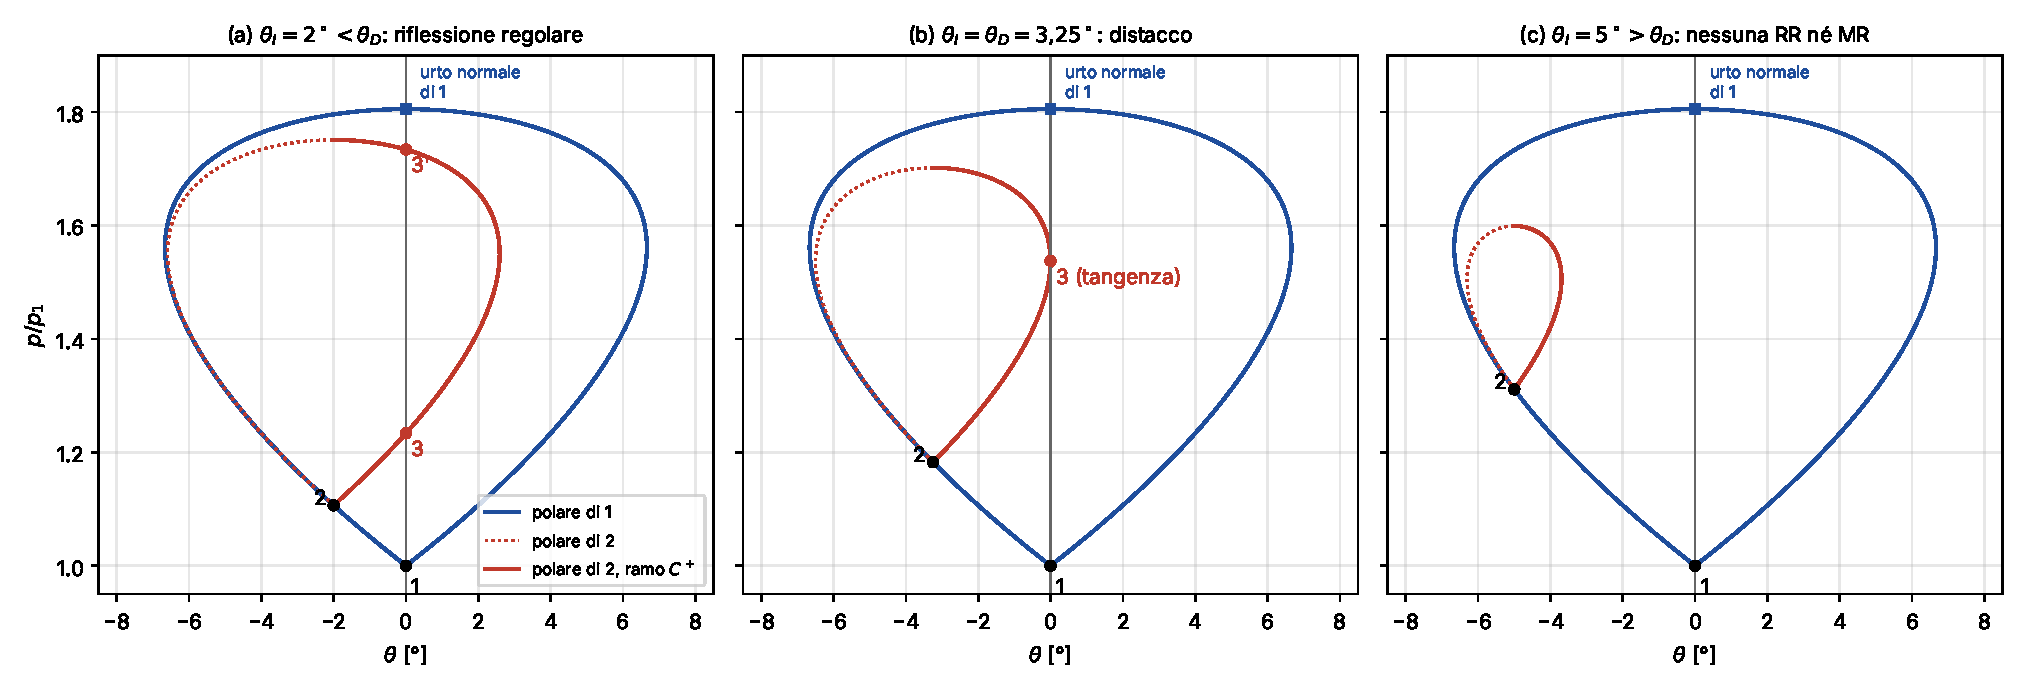
\includegraphics[width=\textwidth]{p_theta.pdf}
  \caption{Piano $p$--$\theta$: polare di 1 (blu), polare di 2 (rosso; a tratto continuo il ramo $\Cp$ utile al
  riflesso). (a) RR: intersezioni 3 (debole) e 3$'$ (forte) con l'asse $\theta=0$. (b) Distacco: polare di 2
  tangente all'asse. (c) Oltre il distacco: la polare di 2 non raggiunge l'asse ed è interna alla polare di 1.}
  \label{fig:ptheta}
\end{figure}
Nella figura~\ref{fig:ptheta} le polari partono dal punto $(0,1)$ e non dall'origine. In (a) si legge la procedura
della RR: dal punto 1 lungo il ramo debole della polare di 1 fino a 2, poi lungo la polare di 2 fino all'asse
$\theta=0$. Da (a) a (c) la polare di 2 si stringe, perché $M_2$ diminuisce: in (b) è tangente all'asse, in (c) non
lo raggiunge più. In tutti e tre i casi resta sotto il ramo forte della polare di 1: nessun punto triplo possibile.

\begin{figure}[H]
  \centering
  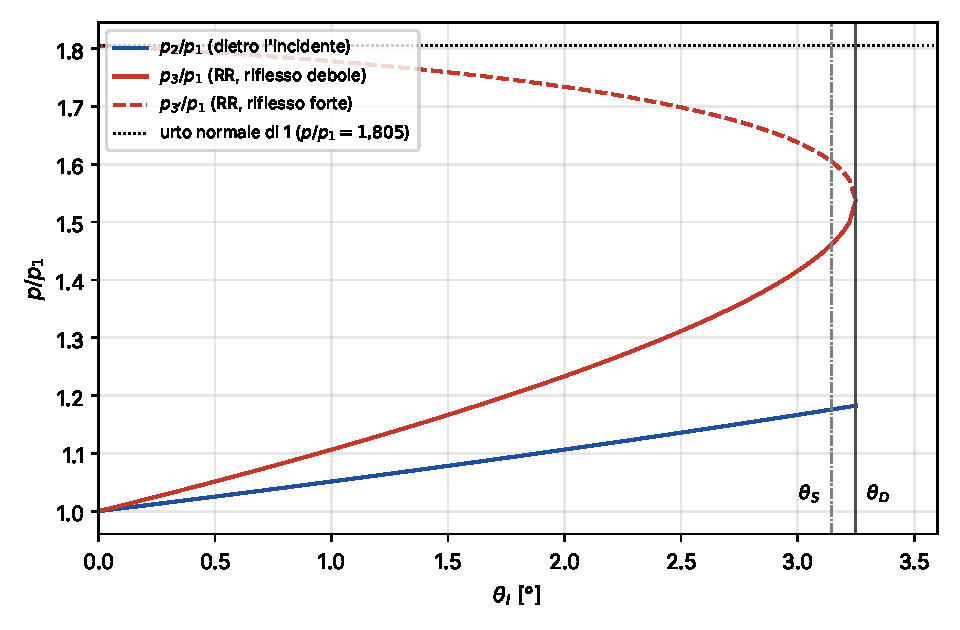
\includegraphics[width=0.62\textwidth]{p_parete.pdf}
  \caption{Pressioni dietro l'incidente e a parete per la RR, al variare di $\theta_I$; in punteggiato la pressione
  dell'urto normale di 1.}
  \label{fig:pparete}
\end{figure}
La figura~\ref{fig:pparete} mostra che il ramo debole e quello forte della RR si congiungono a $\theta_D$, dove
termina la RR, e che $p_3$ resta sempre sotto $p_{n1}=1{,}805$: il criterio di von Neumann non è mai soddisfatto.
Le pressioni coprono un intervallo piccolo (fra 1 e 1,8), quindi basta la scala lineare.

\begin{figure}[H]
  \centering
  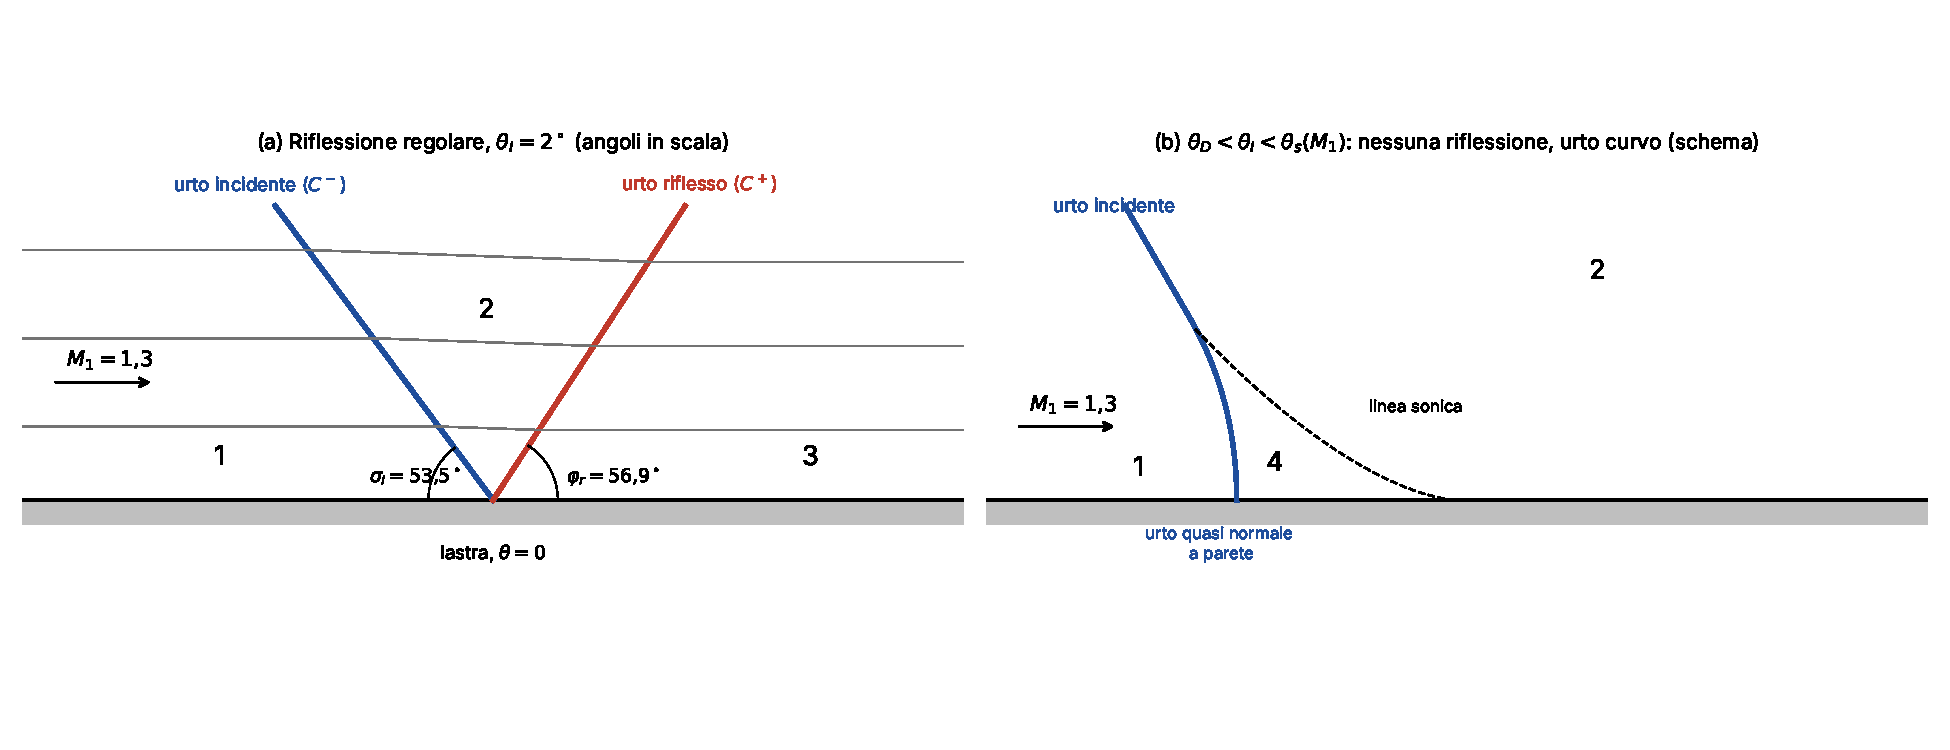
\includegraphics[width=\textwidth]{campo.pdf}
  \caption{Piano fisico. (a) RR a $\theta_I=\ang{2}$, angoli e linee di corrente in scala. (b) Oltre il distacco:
  urto incidente che si incurva e incide perpendicolarmente la lastra, con sacca subsonica 4 (qualitativo).}
  \label{fig:campo}
\end{figure}
Nella figura~\ref{fig:campo}(a) le linee di corrente piegano di \ang{2} verso la lastra attraversando l'incidente e
tornano orizzontali attraverso il riflesso, più inclinato sulla lastra dell'incidente. In (b) l'urto si raccorda alla
lastra con un tratto quasi normale: non c'è urto riflesso né punto triplo; a valle la corrente subsonica 4 riaccelera
e si raccorda con la regione 2 attraverso la linea sonica.

\begin{figure}[H]
  \centering
  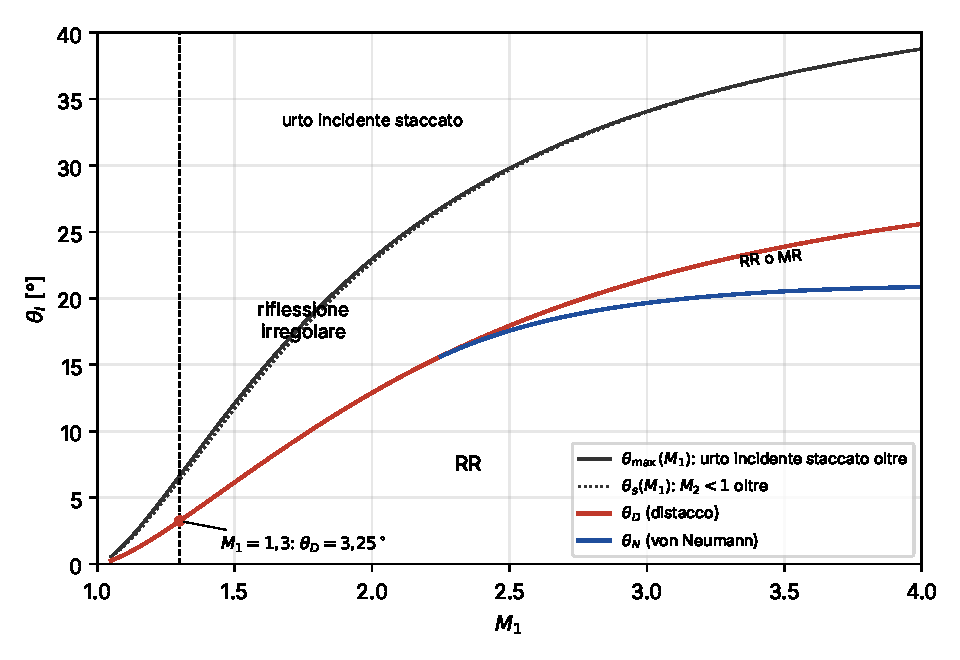
\includegraphics[width=0.62\textwidth]{diagramma_M_theta.pdf}
  \caption{Piano $\theta_I$--$M_1$: deviazione massima e sonica di 1, criteri di distacco $\theta_D$ e di von Neumann
  $\theta_N$; tratteggiata la retta $M_1=1{,}3$.}
  \label{fig:diagr}
\end{figure}
La figura~\ref{fig:diagr} colloca il caso nel quadro generale: $\theta_N$ esiste solo per $M_1\gtrsim2{,}2$, dove si
apre la regione di doppia soluzione fra $\theta_N$ e $\theta_D$; a $M_1=1{,}3$ la retta verticale incontra solo
$\theta_D=\ang{3.25}$ e poi, a pochi gradi di distanza, $\theta_s$ e $\theta_{\max}$.

%==============================================================================
\section{Discussione fisica}
\begin{itemize}
\item A Mach basso tutte le soluzioni stanno in pochi gradi di deviazione: basta un urto incidente debole
  ($p_2/p_1\approx1{,}18$) per rendere impossibile la RR, perché il riflesso parte da $M_2\approx1{,}17$, la cui
  polare ammette meno di \ang{3.3} di deviazione.
\item La RR si osserva fino a $\theta_D$, ma da $\theta_S$ in poi la regione 3 è subsonica: le perturbazioni di valle
  (per esempio la spalla del cuneo che genera l'incidente) possono risalire fino al punto di riflessione, quindi la
  transizione reale avviene fra $\theta_S$ e $\theta_D$, intervallo qui di appena \ang{0.1}.
\item La MR a tre urti richiede che la polare riflessa esca dalla polare incidente: a $M_1=1{,}3$ la polare
  riflessa è sempre contenuta in quella incidente, quindi oltre il distacco non c'è riflessione e l'urto incidente
  si incurva fino a incidere perpendicolarmente la lastra. Le misure reali in questo regime mostrano un urto che
  si raccorda con continuità alla parete, con una debole compressione riflessa che si dissolve, invece di un punto
  triplo netto.
\item Non c'è isteresi: mancando $\theta_N$, la configurazione dipende solo da $\theta_I$ e non dal verso in cui lo
  si fa variare, a differenza di quanto accade per $M_1\gtrsim2{,}2$.
\item Il riflesso non segue la legge ottica ($\varphi_R\ne\sigma_I$): è più inclinato e più intenso perché deve dare
  la stessa deviazione partendo da un Mach minore.
\item Lo strato limite sulla lastra, trascurato, a questi Mach interagisce fortemente con l'urto (la sua parte
  subsonica trasmette la sovrapressione a monte) e può separare: è il limite principale del modello non viscoso.
\end{itemize}

\end{document}
